\begin{problem}{Someday in the rain}{Someday in the rain.in}{Someday in the rain.out}{1 seconds}

平凡的日常。

春日不知道用了什么方法获取到了电器街老板们的赞助,电器街上的每一家都答应赠送春日一种电器,还可以选择一家店免费租用他们的仓库。而搬运电器这个光荣的使命自然而然地就落到了你的身上。

你需要选择一家店作为仓库,任务是把所有的电器都搬回仓库,遗憾的是由于电器实在是太沉了,每一次只能搬一台电器。已知电器街所有店之间的道路恰好构成一棵无根树。那么现在任务就变得很简单了,选择哪家电器作为仓库可以使搬完所有电器的路程最短呢(如果有多个店铺满足要求就输出编号最小的,为什么呢,因为我不想写SPJ呀)。

\InputFile

第一行一个正整数 $n (2 \leq n \leq 10^6)$ ,表示电器街上店的数量。

接下来 $n-1$ 行,每行包含三个正整数 $x,y,v (1 \leq x,y \leq n,1 \leq v \leq 10^5)$ ,表示店 $x$ 与店 $y$ 之间有一条长为 $v$ 的道路。 

\OutputFile

第一行一个正整数 $X$ ,表示选择 $X$ 店作为仓库时路程总和最短(有多个 $X$ 时输出最小的那一个)。

第二行一个整数 $S$ ,表示此时的总路程。

\Example
\begin{example}
\exmp{
5
1 2 9
1 3 1
3 4 2
3 5 4
}{
3
34
}%
\end{example}
\begin{center}
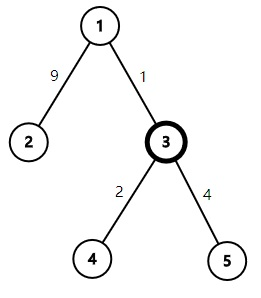
\includegraphics[width=0.3\textwidth]{pics/H.jpg}
\end{center}
\end{problem}
